\documentclass[12pt,a4paper]{article}
\usepackage{hw}

\graphicspath{ {.} }
\setlength\parindent{0pt}

\begin{document}
    \qtitle{9.1}
    Let $\pmb{\mu}=\newvec{\mu_1\\\mu_2}$ and $\pmb{\Sigma}=\newvec{\sigma_1^2 & \rho\sigma_1\sigma_2\\\rho\sigma_1\sigma_2&\sigma_2^2 }$, then \\
    $p(\mathbf{x}|\theta_1)=\cfrac{exp(-\frac{1}{2}(\mathbf{x}-\pmb{\mu})^T\pmb{\Sigma}^{-1}(\mathbf{x}-\pmb{\mu})))}{\sqrt{(2\pi)^2|\pmb{\Sigma}|}}\Longleftrightarrow\\
    p(x_1,x_2|\theta_1)=\cfrac{1}{2\pi\sigma_1\sigma_2\sqrt{1-\rho^2}}exp(-\cfrac{1}{2(1-\rho^2)}[\cfrac{(x_1-\mu_1)^2}{\sigma_1^2}+\cfrac{(x_2-\mu_2)^2}{\sigma_2^2}-\cfrac{2\rho(x_1-\mu_1)(x_2-\mu_2)}{\sigma_1\sigma_2}])$

    If $x_1$ and $x_2$ are independent, which means $\rho=0$, then $\Sigma=\newvec{\sigma_1^2&0\\0&\sigma_2^2}$. \\
    $p(x_1,x_2|\theta_1)=p(x_1|\theta_1)*p(x_2|\theta_1)\\=\cfrac{1}{2\pi\sigma_1\sigma_2}exp(-\cfrac{1}{2}[\cfrac{(x_1-\mu_1)^2}{\sigma_1^2}+\cfrac{(x_2-\mu_2)^2}{\sigma_2^2}])$

    \newpage
    \qtitle{9.2}
    To simplify quandratic discriminant function, if $\theta_1$ and $\theta_2$ have similar distribution, that is $\mathbf{K_1=K_2}\rightarrow\\
    \mathbf{S}_w=Pr(\theta_1)\mathbf{K_1}+Pr(\theta_2)\mathbf{K_2}=0.5(\mathbf{K_1+K_2})=\mathbf{K_1}=\mathbf{K_2}$

    Given 9.21, \\
    $L(\mathbf{x})=(x-\pmb{\mu_1})^T\mathbf{K}_1^{-1}(x-\pmb{\mu_1})-(x-\pmb{\mu_2})^T\mathbf{K}_2^{-1}(x-\pmb{\mu_2})+\ln\cfrac{det\mathbf{K_1}}{det\mathbf{K_2}} \overset{\theta_2}{\underset{\theta_1}{\lessgtr}}t\Longleftrightarrow\\
    L(\mathbf{x})\simeq (x-\pmb{\mu_1})^T\mathbf{S}_w^{-1}(x-\pmb{\mu_1})-(x-\pmb{\mu_2})^T\mathbf{S}_w^{-1}(x-\pmb{\mu_2})\\
    =\mathbf{x}^T\mathbf{S}_w^{-1}\mathbf{x}-2\pmb{\mu_1}^T\mathbf{S}_w^{-1}\mathbf{x}+\pmb{\mu_1}^T\mathbf{S}_w^{-1}\pmb{\mu_1}-\mathbf{x}^T\mathbf{S}_w^{-1}\mathbf{x}+2\pmb{\mu_2}^T\mathbf{S}_w^{-1}\mathbf{x}-\pmb{\mu_2}^T\mathbf{S}_w^{-1}\pmb{\mu_2}\\
    =2(\pmb{\mu_2}-\pmb{\mu_1})\mathbf{S}_w^{-1}\mathbf{x}+\pmb{\mu_1}^T\mathbf{S}_w^{-1}\pmb{\mu_1}-\pmb{\mu_2}^T\mathbf{S}_w^{-1}\pmb{\mu_2} \overset{\theta_2}{\underset{\theta_1}{\lessgtr}}t\Longleftrightarrow\\
    2(\pmb{\mu_2}-\pmb{\mu_1})\mathbf{S}_w^{-1}\mathbf{x} \overset{\theta_2}{\underset{\theta_1}{\lessgtr}}t+\pmb{\mu_2}^T\mathbf{S}_w^{-1}\pmb{\mu_2}-\pmb{\mu_1}^T\mathbf{S}_w^{-1}\pmb{\mu_1}$

    This is LDA form in equation 9.22, with $\mathbf{a}^T=2(\pmb{\mu_2}-\pmb{\mu_1})\mathbf{S}_w^{-1}$ and $b=t+\pmb{\mu_2}^T\mathbf{S}_w^{-1}\pmb{\mu_2}-\pmb{\mu_1}^T\mathbf{S}_w^{-1}\pmb{\mu_1}$

    \newpage
    \qtitle{9.3}
    \textbf{a.}
    Because $\mathbf{K_1=K_2}$, $\sigma_{\theta_1}=\sigma_{\theta_2};\rho_{\theta_1}=\rho_{\theta_2}$. Replace the code with the following lines:
    \begin{lstlisting}
    N=1000;
    mx1=0;my1=0;sx1=40;sy1=25;r1=-0.7;
    mx2=0;my2=40;sx2=40;sy2=25;r2=-0.7;
    ...
    TPF(i)=1e-3*C2;FPF(i)=1e-3*C1;
    ...
    \end{lstlisting}
    \begin{figure}[!ht]
        \includegraphics*[width=\textwidth]{hw9_3a.png}
        \caption{Blue triangles belong to  $\theta_2$ and red dots are $\theta_1$}
    \end{figure}
    The AUC values is 0.9463. 

    For $J_h$, $\mathbf{S}_w^{-1}=\newvec{0.0012&0.0014\\0.0014&0.0031}$; \\ $\overline \mu=\sum_{i=1}^C\mu_i*0.5=\newvec{0\\0}*0.5+\newvec{0\\40}*0.5=\newvec{0\\20}\rightarrow\\
    \mathbf{S}_b=\sum_{i=1}^C(\mathbf{\mu_i-\overline \mu})(\mathbf{\mu_i-\overline \mu})^T*0.5=\newvec{0&0\\0&400}$\\
    Therefore, $J_h=tr(\mathbf{S}_w^{-1}\mathbf{S}_b)=1.255$

    \vspace{0.3cm}
    For $B$, $B(\mu)=\cfrac{1}{8}(\mu_2-\mu_1)^T\mathbf{S}_w^{-1}(\mu_2-\mu_1)=\cfrac{1}{8}\newvec{0&40}\mathbf{S}_w^{-1}\newvec{0\\40}=0.6275$, distance from the difference between class means;\\
    $B(\mathbf{K})=\cfrac{1}{2}ln(\cfrac{det(\mathbf{S}_w)}{\sqrt{det(\mathbf{K_1})det(\mathbf{K_2})}})=0$, because their covariance matrices are indentical. Therefore, $B=B(\mu)+B(K)=0.6275$

    \textbf{b.} Change $\mu_2=\newvec{0\\40}\rightarrow\newvec{0\\20}$. $\theta_1$ and $\theta_2$ overlap more, so their separability decreases, indicating $J-h$, AUC, and $B$ would decrease.

    \begin{figure}[!ht]
        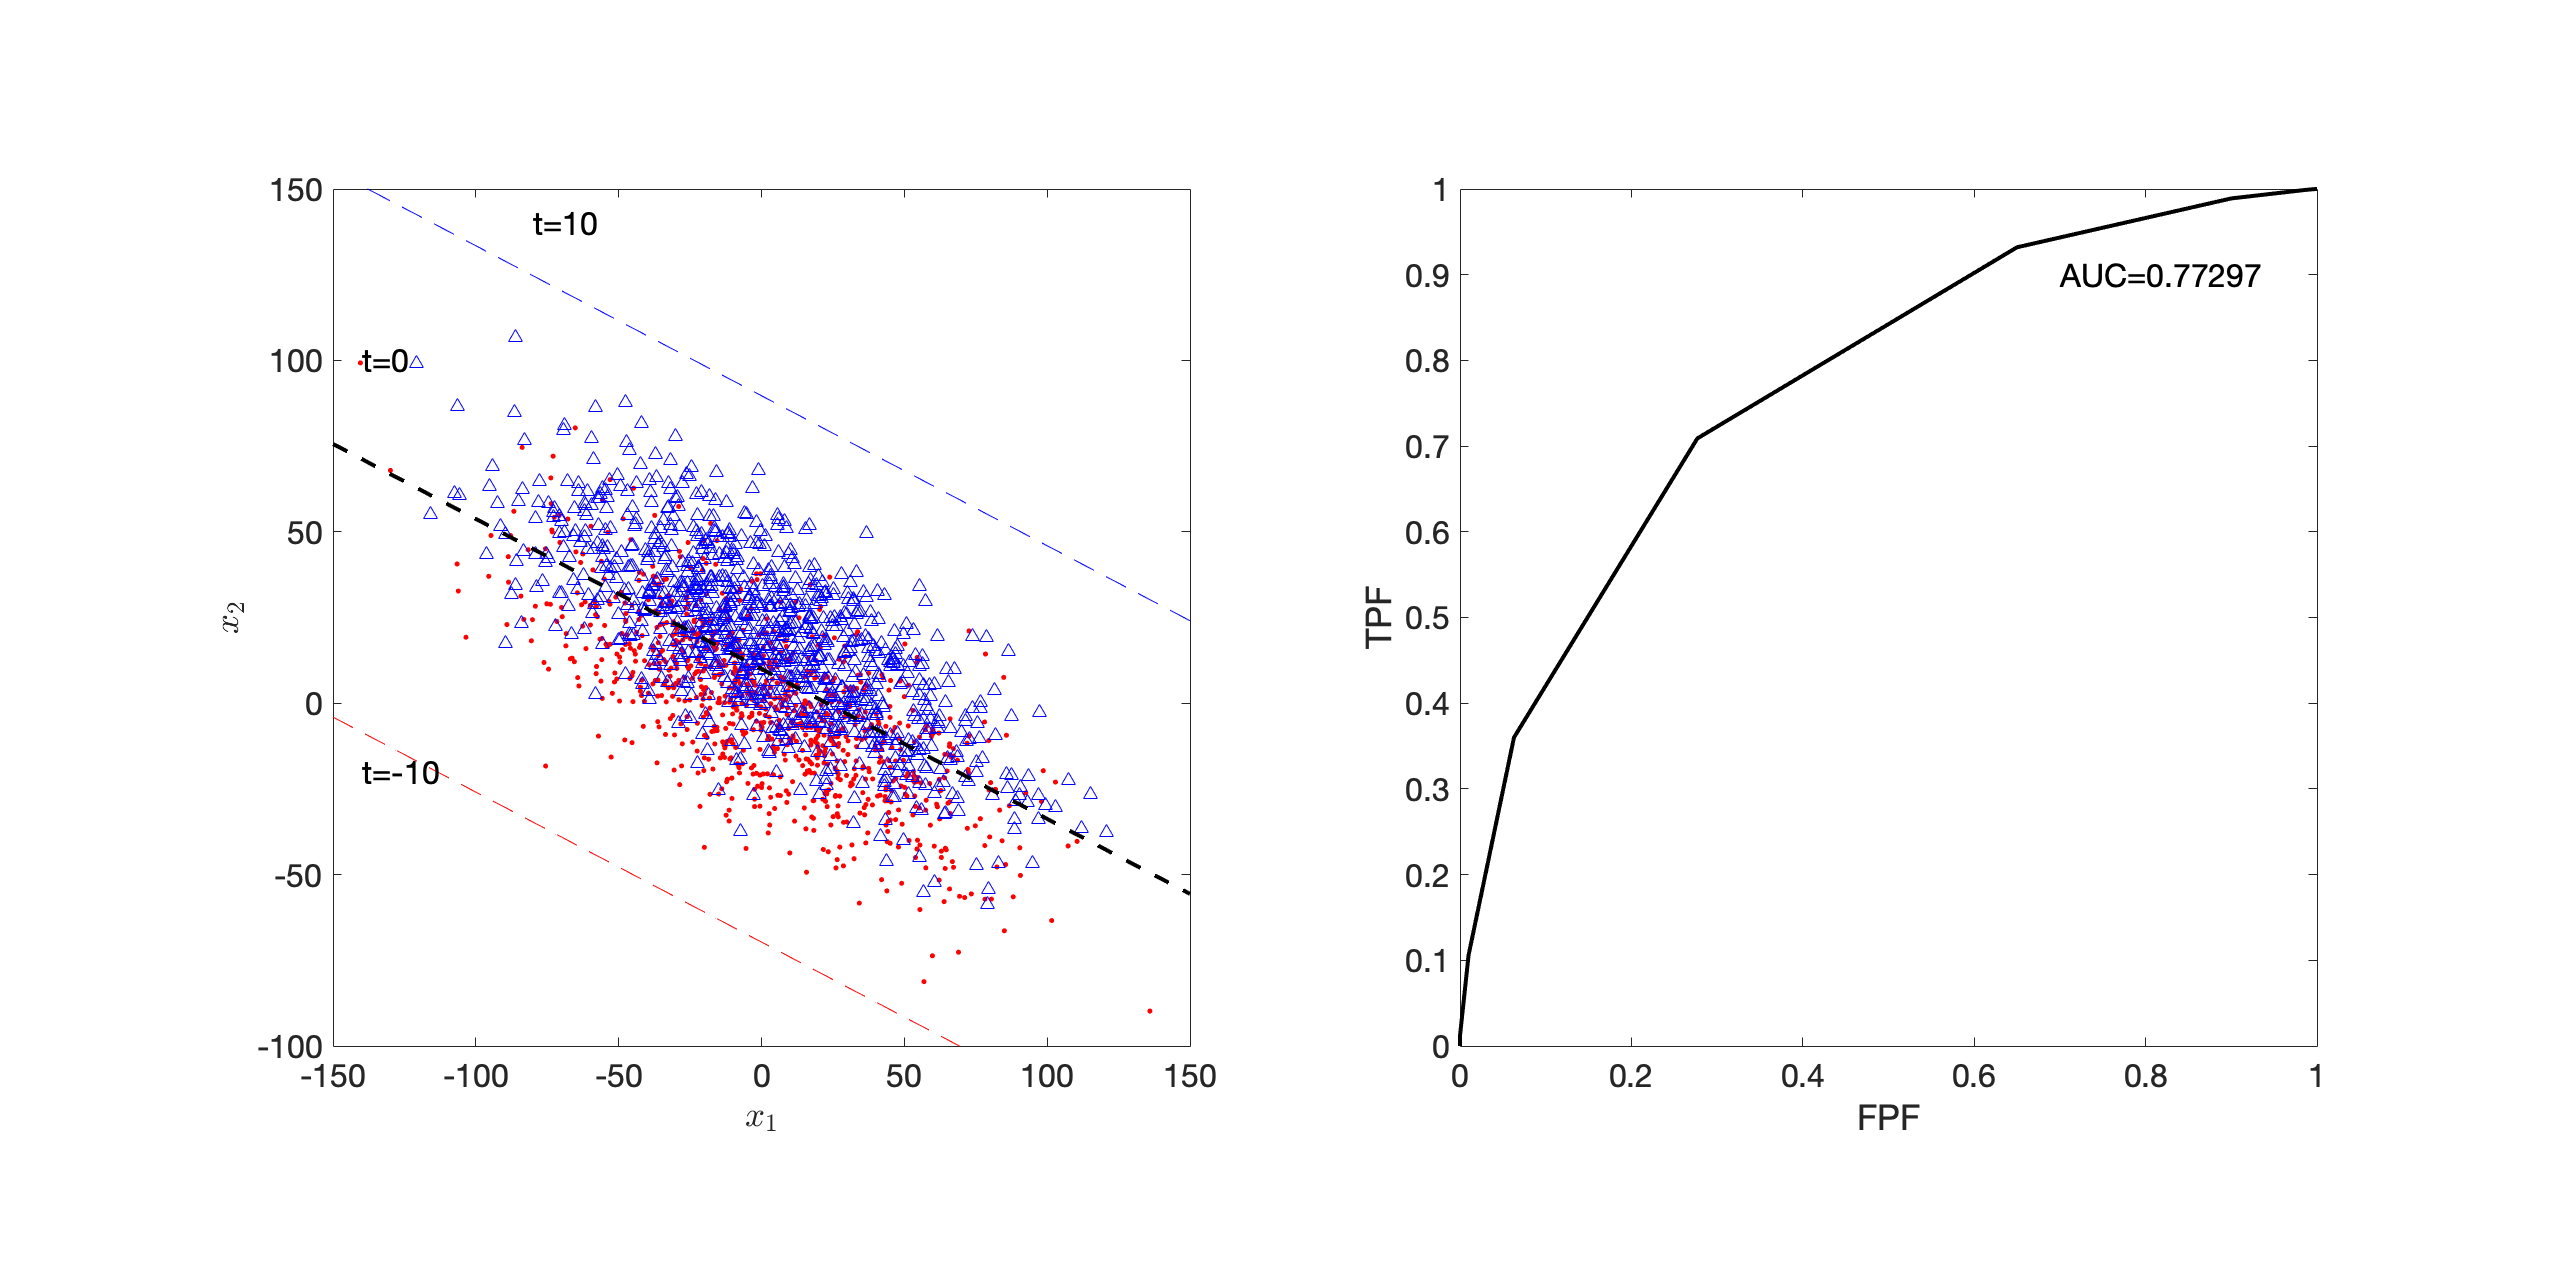
\includegraphics[width=\textwidth]{hw9_3b.png}
    \end{figure}
    AUC=0.773; $J_h$=0.3137; $B$=0.1569
    
    \textbf{c.} 
    \begin{figure}[!ht]
        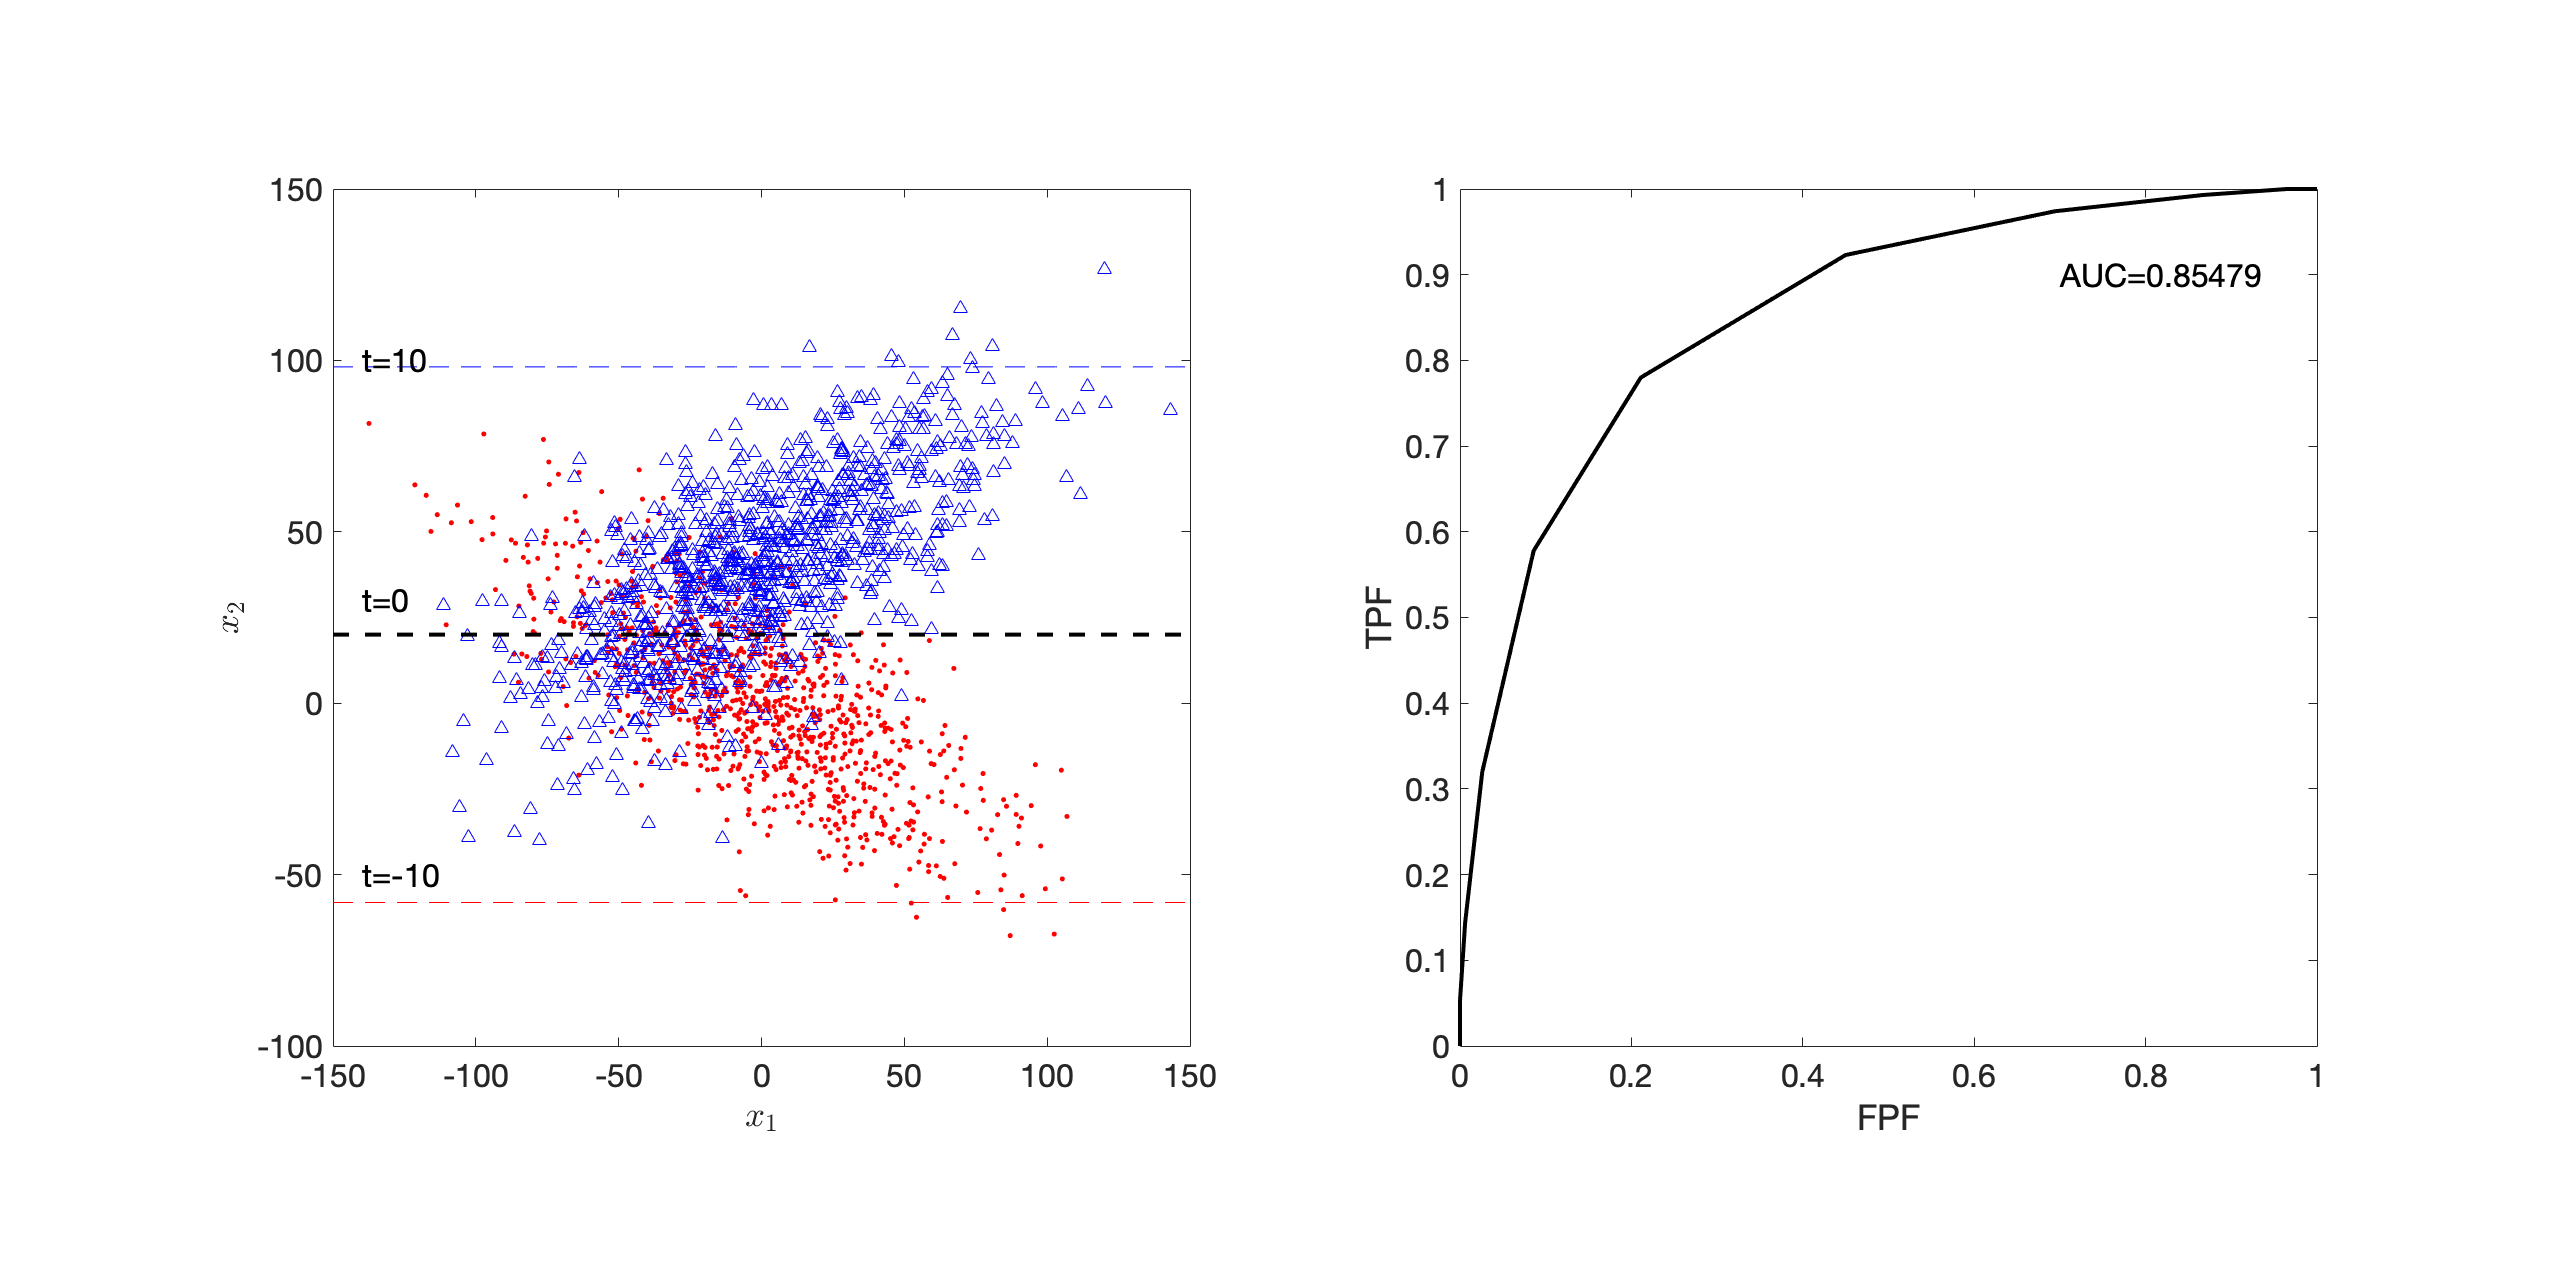
\includegraphics[width=\textwidth]{hw9_3c.png}
    \end{figure}
    As shown in the figure, $\theta_1$ and $\theta_2$ are symmetric along the horizontal axis. Since their overlap also increases, $Jh$ and AUC would still decrease.

    AUC=0.8548; $J_h=0.64$; For $B$, now $K_1\neq K_2$, so $B(K)\neq 0$. $B(K)=0.3367;B(\mu)=0.32\rightarrow B=0.6567$
    
    \textbf{d.}    
    Change $N$ from 10 to 10,000.$N=10\rightarrow AUC=0.96;\\
    N=100\rightarrow AUC=0.944;\\
    N=1000\rightarrow AUC=0.948;\\
    N=10000\rightarrow AUC=0.943$.\\
    As shown in the figure, the AUC value changes little when sample number increases. This is because the dots are independently generated from the bivariate normal distribution and their labels are determined by threshold $t$ directly. Whether the dot is tagged positive or negative is only determined by the distribution and the threshold, having nothing to do with the number of samples. 

    Similarly, since $J_h$ and $B$ only determined by $\mu$ and covariance matrix $K$, which are not immutable when changing the number of samples. Their values keep same as shown in \textbf{a}. 
    \begin{figure}[!ht]
        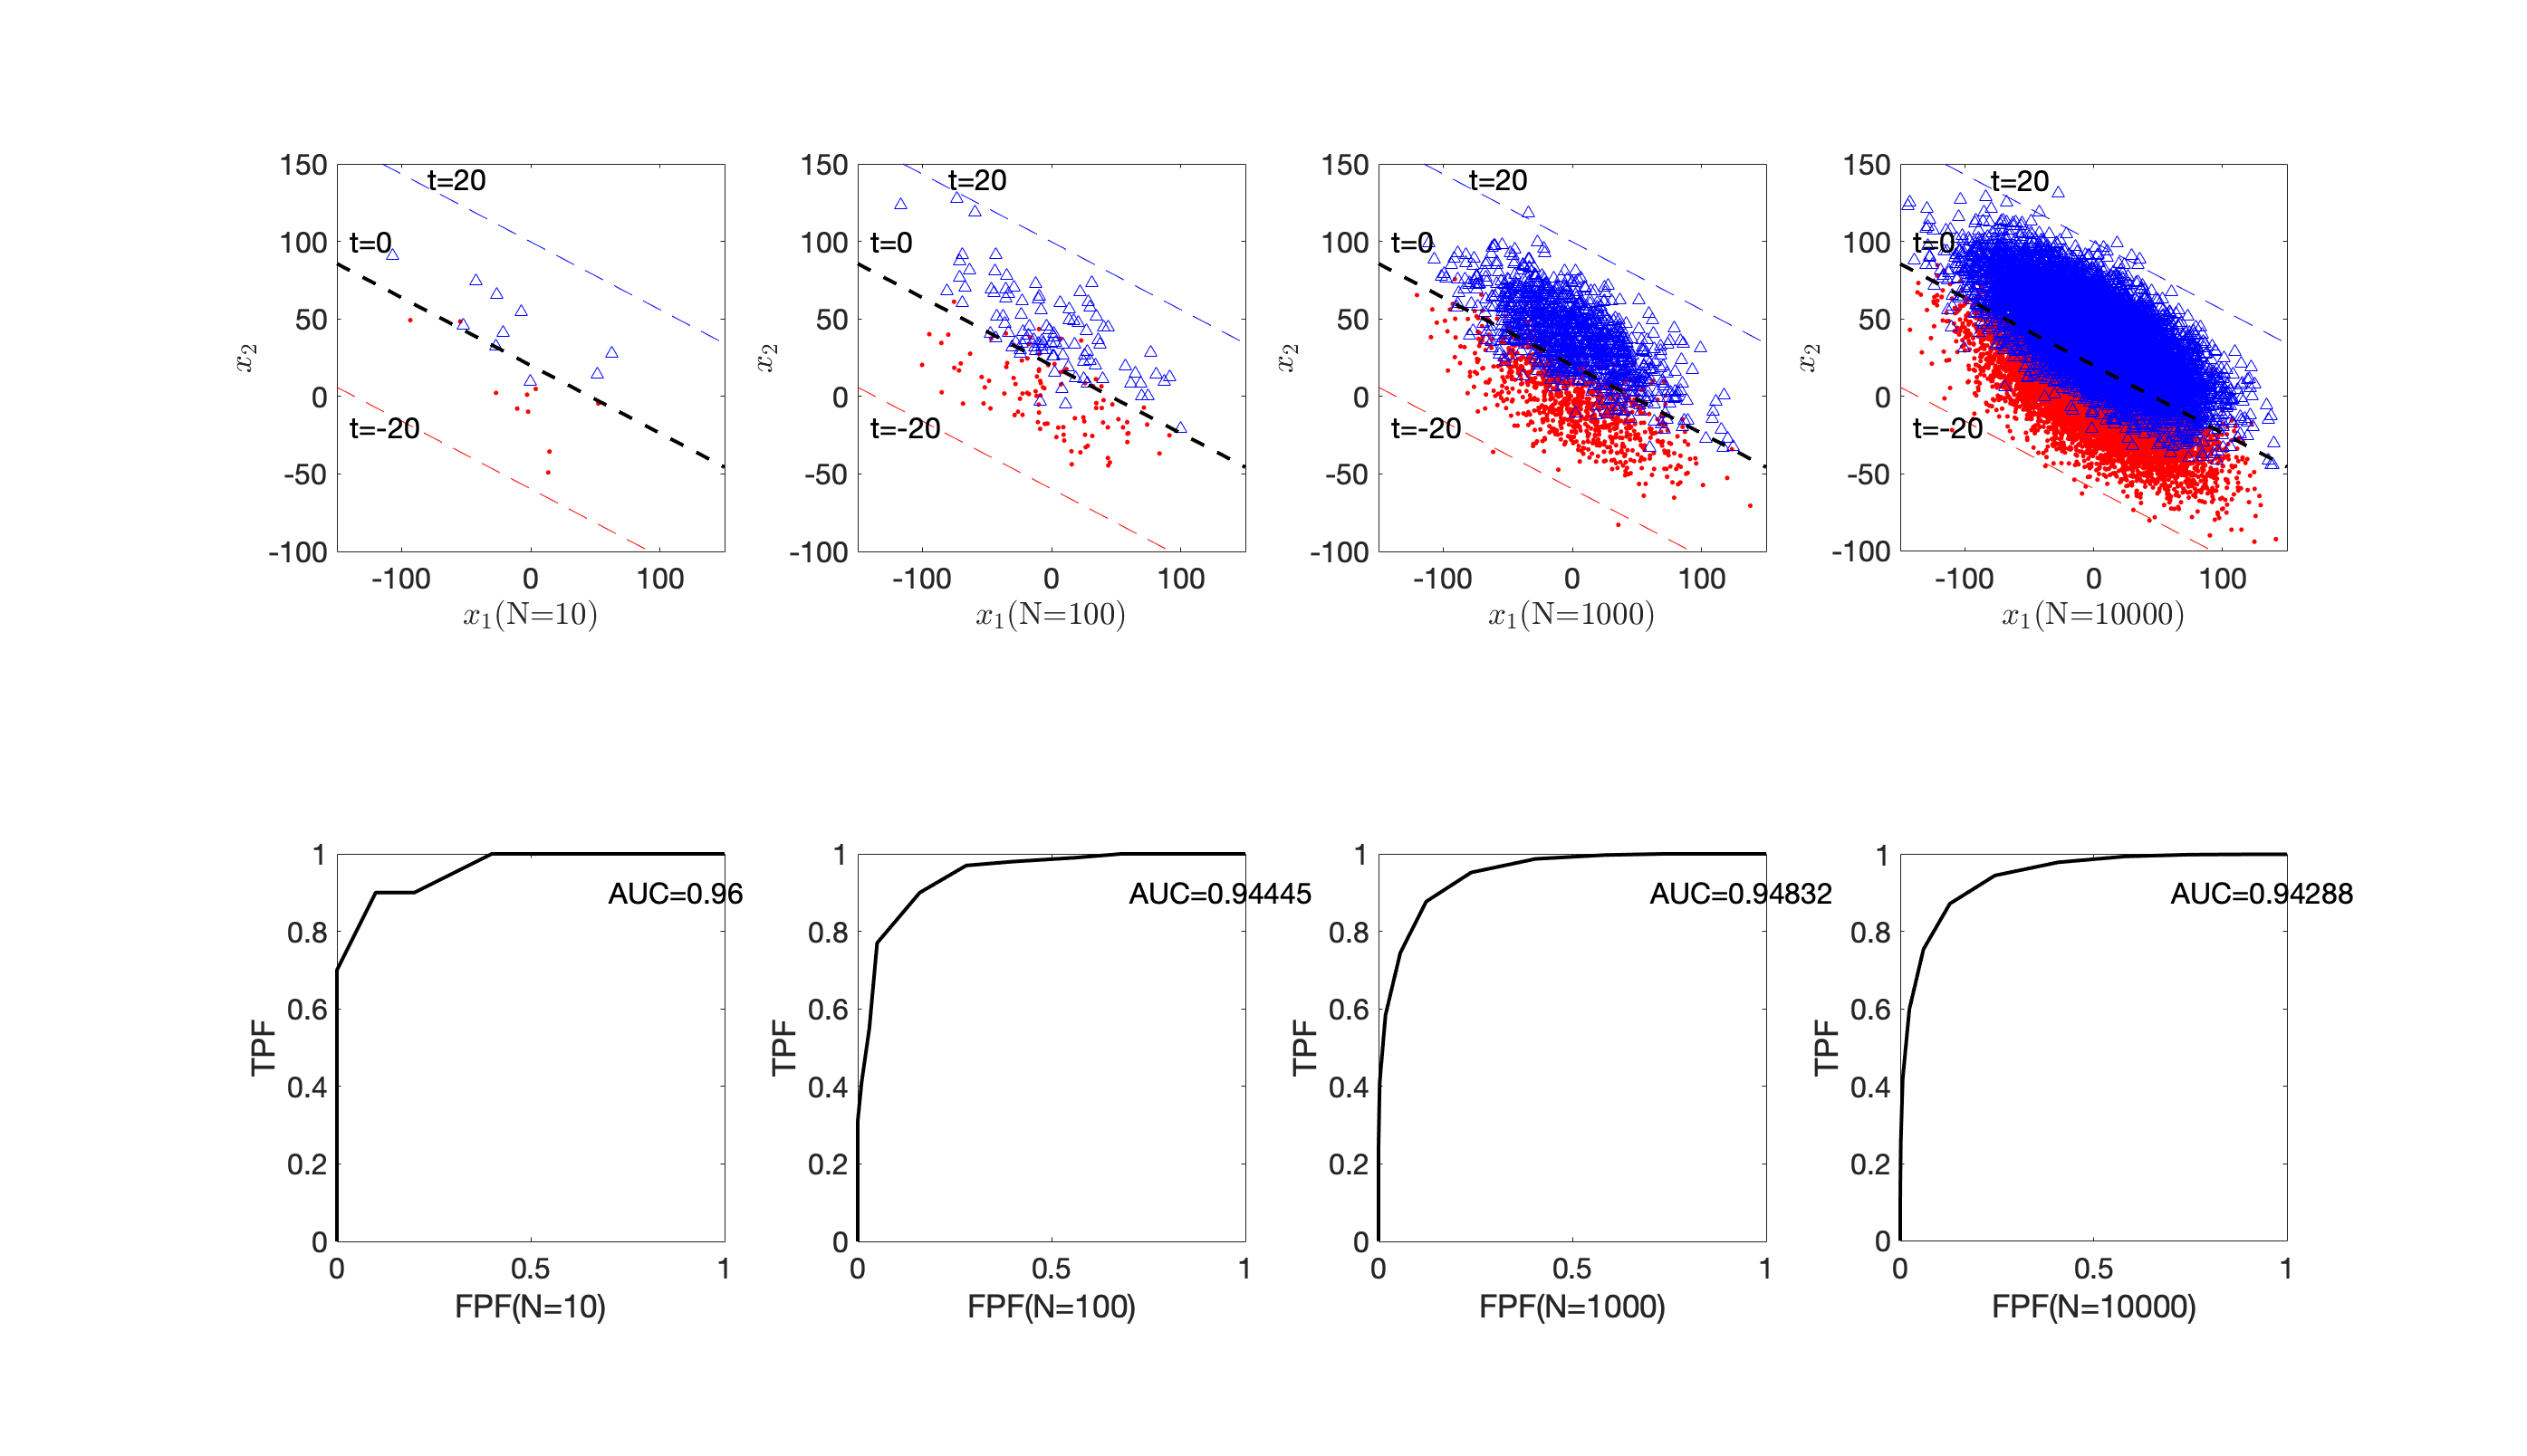
\includegraphics[width=\textwidth]{hw9_3d.png}
    \end{figure}

    \newpage
    \qtitle{9.4}
    Modify the code used in the linear discriminant section as follows:
    \begin{lstlisting}[basicstyle=\tiny]
    clear all;N=1000;
    scaffold=1/N;
    mx1=0;my1=0;mz1=-10;sx1=40;sy1=40;sz1=10;r12=0;r13=0.4;r23=0.4;
    mx2=0;my2=40;mz2=15;sx2=40;sy2=40;sz2=10;
    m1=ones(N,2);m1(:,1)=m1(:,1)*mx1;m1(:,2)=m1(:,2)*my1;m1(:,3)=mz1;
    m2=ones(N,2);m2(:,1)=m2(:,1)*mx2;m2(:,2)=m2(:,2)*my2;m2(:,3)=mz2;
    M1=[mx1;my1;mz1];M2=[mx2;my2;mz2];
    K1=[sx1^2 r12*sy1*sx1 r13*sx1*sz1;r12*sx1*sy1 sy1^2 r23*sy1*sz1; r13*sx1*sz1 r23*sy1*sz1 sz1^2];
    K2=K1;
    Swi=2*eye(3)/(K1+K2);
    X1=mvnrnd(m1,K1);X2=mvnrnd(m2,K2);
    figure('Position', [0 0 1280 640]);
    subplot(1,2,1);
    scatter3(X1(:,1),X1(:,2),X1(:,3), 'r');axis square; hold on;
    scatter3(X2(:,1),X2(:,2),X2(:,3), 'b');axis square; hold on;
    t=-60:2:20;Nt=length(t);TPF=zeros(1,Nt);FPF=TPF;
    px=[-150 150 150 -150];py=[-150 -150 150 150];
    for i=1:Nt
        a=2*(M2-M1)'*Swi;
        b=t(i)+M2'*Swi*M2-M1'*Swi*M1;
        pz=(b-a(1)*px-a(2)*py)/a(3);
        C1=0;C2=0;
        for j=1:N
            if (X1(j,3)>(b-a(1)*X1(j,1)-a(2)*X1(j,2))/a(3))
                C1=C1+1;
            end
            if (X2(j,3)>(b-a(1)*X2(j,1)-a(2)*X2(j,2))/a(3))
                C2=C2+1;
            end
        end
        TPF(i)=scaffold*C2;FPF(i)=scaffold*C1;
        if(t(i)==0);patch(px,py,pz, 'k','faceAlpha', 0.2);text(150, 150, 25, 't=0', 'fontsize', 16);end
    end
    subplot(1,2,2);
    plot(FPF,TPF,'k','linewidth',2);axis square;
    AUC=trapz(FPF,TPF);
    text(0.7,0.9,"AUC="+num2str(-AUC), 'fontsize', 16);
    \end{lstlisting}

    Then when $t=0$, the separate plane determined by LDA is shown in the following figure:
    \begin{figure}[!ht]
        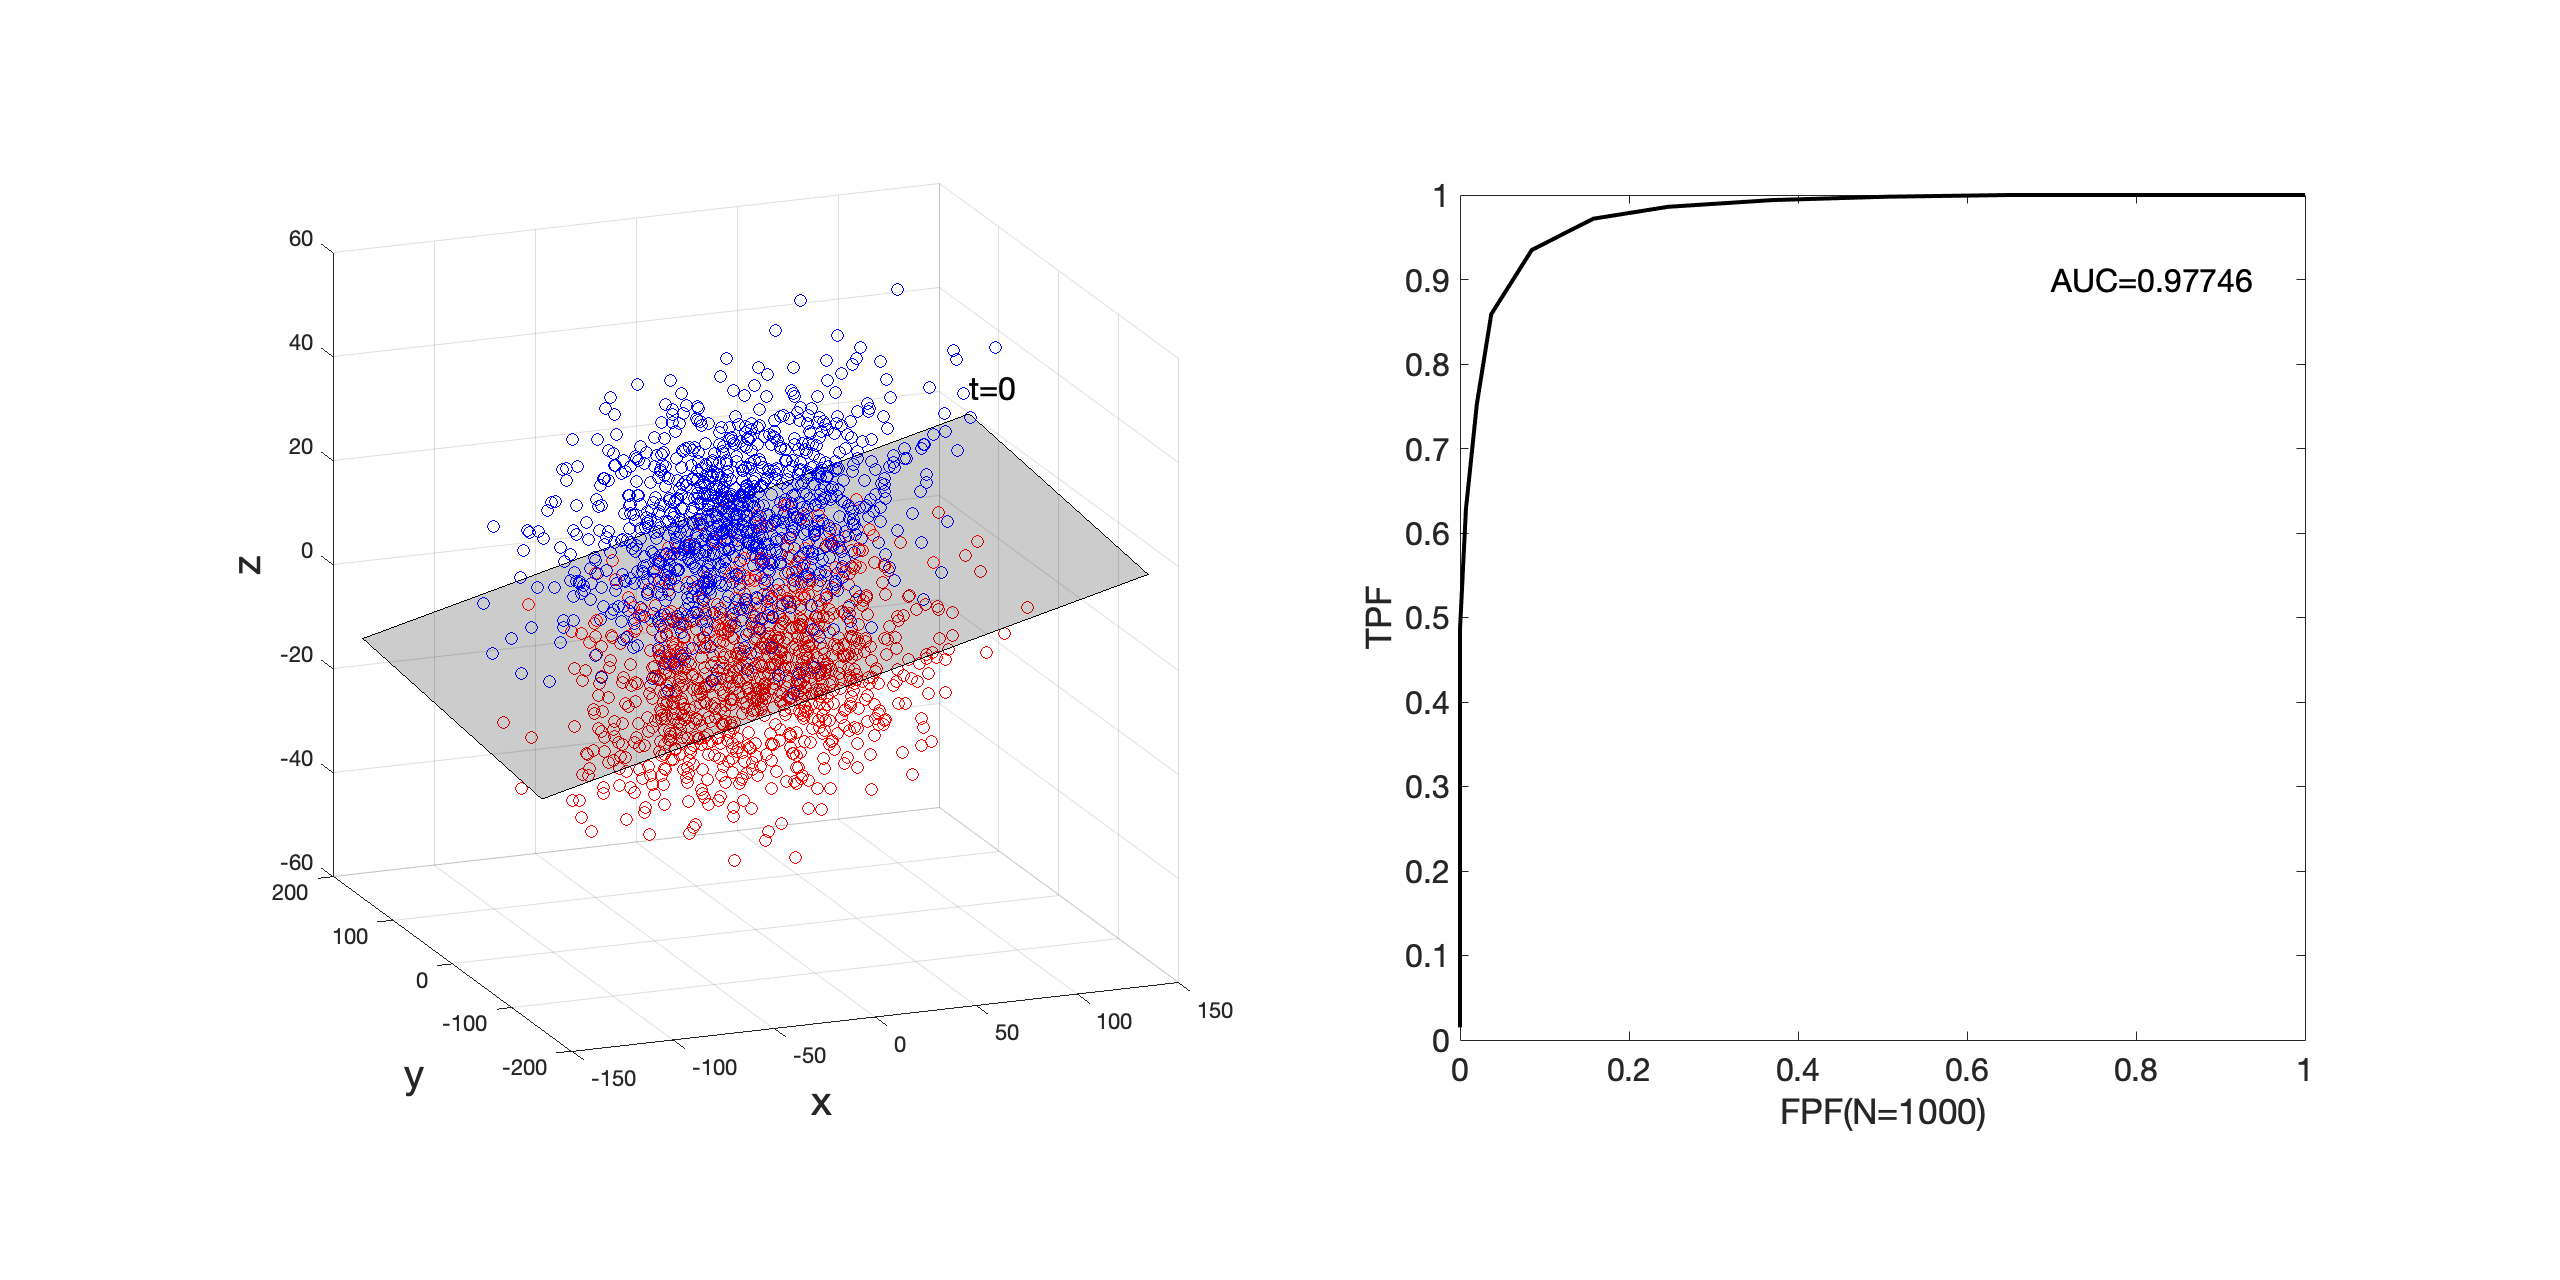
\includegraphics[width=\textwidth]{hw9_4.png}
    \end{figure}

    $J_h=1.8713;B=B_\mu=0.9357;AUC=0.9775$. The separability metrics, where $J_h$ is larger than 1 and AUC is almost close to 1, indicating the 2 classes are well separated by the $t=0$ decision plane. It coresponds to the situation that points of these 2 classes overlap little.
    
    \newpage
    \qtitle{9.5}
    Apply the following code to do 2-classes kmeans clustering:
    \begin{lstlisting}
    options=statset('Display', 'final');
    [idx, C] = kmeans(X, 2, 'replicates', 3, 'options', options);
    ic =0;
    for j=1:length(X1)
        if idx(j) ~= 1;ic=ic+1;end
    end
    for k=length(X1)+1:length(X)
        if idx(k) ~= 2;ic=ic+1;end
    end
    subplot(1,2,2);
    plot(X(idx==1,1), X(idx==1,2),'ro', 'markersize',6);hold on;
    plot(X(idx==2,1),X(idx==2,2),'b+', 'markersize',6);
    plot(C(:,1),C(:,2),'kx','markersize',12,'linewidth',3);hold off
    \end{lstlisting}

    Then we would get the 2-classes clustering result.
    \vspace{-0.5cm}
    \begin{figure}[!ht]
        \centering
        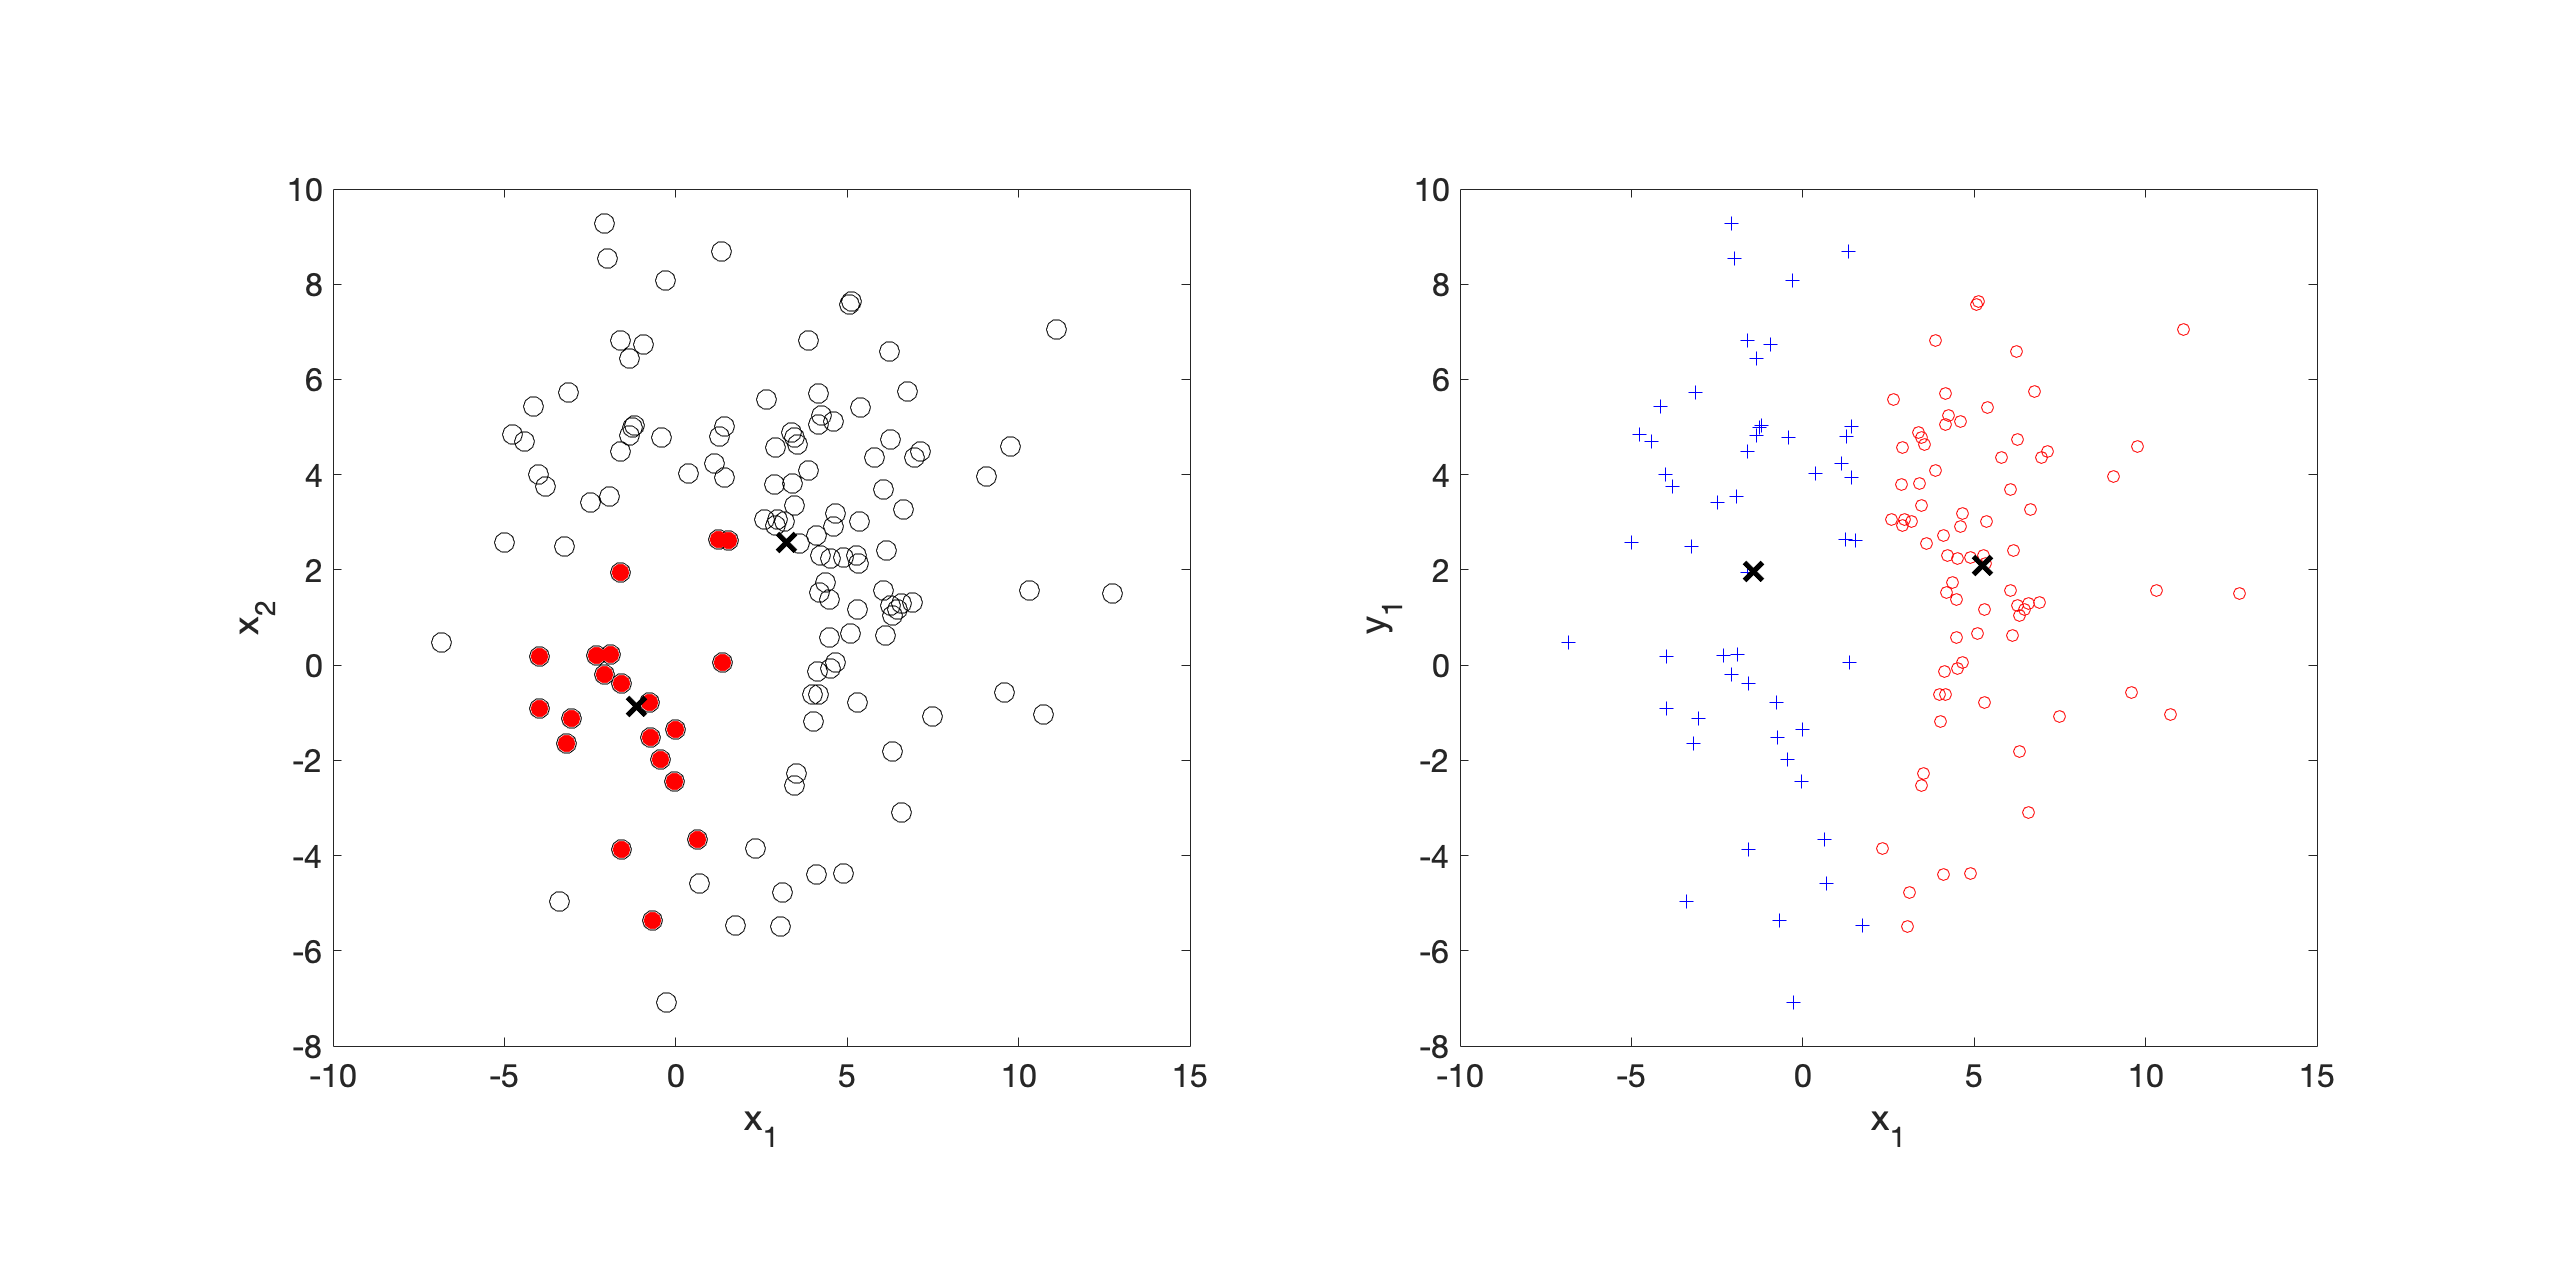
\includegraphics[width=0.85\textwidth]{hw9_5.png}
        \vspace{-0.5cm}
        \caption{Left figure is the distribution of the 2 classes, where empty circles belong to $\theta_1$ and red circles belong to $\theta_2$; Right figure is the 2-classes kmeans clustering results of the points, where the blue dots (plus) are $\theta_1$ and the red dots (circle) are $\theta_2$. The black bold cross points indicate the center points of each cluster.}
    \end{figure}

    As shown in the previous figure, the centers of unsupervised clusters deviate initial class mean values a lot on $x_2$ axis. This is because $x_2$ points are almost included in $x_1$ distribution. When clustering the points into 2 classes, the decision plane tend to separated the points evenly to minimize sum-squared difference. Therefore, as shown in the right figure above, the decision plane $x_1=2.5$ divides the points into 2 classes, which are almost symmetric along the decision plane. Compared with initial classes where $\theta_1$ has 109 points and $\theta_2$ has 20 points, the cluster $\theta_1'$ has 77 points and cluster $\theta_2'$ has 52 points. There are 32 points are mislabeled, so the error rate is $32/129=0.248$. 
\end{document}